
\question{10}

\noindent
Consider the binary hypothesis testing (Bayesian classification) problem and refer to the following graph (shown below) for the PDF of $Y$ under $H_0$ and $H_1$:

\begin{figure}[htb]
\centering
\centerline{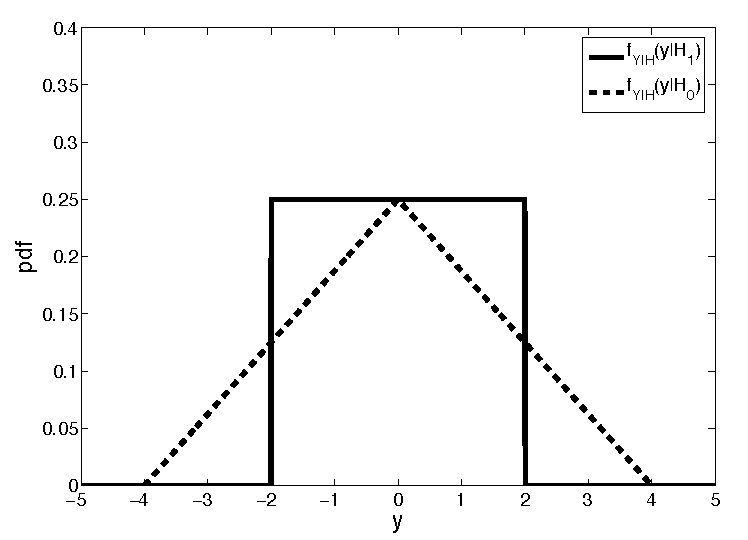
\includegraphics[width=6cm]{bayesdetection.pdf}}
%
\end{figure}

\begin{enumerate}[label=(\alph*)]
\item Using the graph below, write equations (in terms of $y$) for the following likelihoods $f_{Y|H}(y|H_0)$ and  $f_{Y|H}(y|H_1)$
\item For equal priors and uniform costs ($C_{00} = C_{11} = 0$ and $C_{01} = C_{10} = 1$), find the Bayesian decision rule for testing $H_0$ versus $H_1$
\item For part (b), compute the minimum Bayesian risk
\end{enumerate}
